\documentclass[aspectratio=169]{beamer}
\usepackage[utf8]{inputenc}
\usepackage{sansmathfonts}
\usepackage{xcolor}
\usepackage[T1]{fontenc}
\usepackage[ttdefault=true]{AnonymousPro}
% \renewcommand*\familydefault{\ttdefault}
\renewcommand*\familydefault{\sfdefault}
% \usepackage{cmbright}

\usepackage{graphicx}

\graphicspath{
    {themes/gd/images/},
    {images/}
}
\usepackage{themes/gd/beamerthemegd}
\usepackage{themes/gd/beamerinnerthemegd}
\usepackage{themes/gd/beamerouterthemegd}
\usepackage{themes/gd/beamercolorthemegd}


\title{Time In Distributed Systems\\ Pt.1}
% \date[ISPN ’80]{27th International Symposium of Prime Numbers}
\author[Euclid]{Euclid of Alexandria \texttt{euclid@alexandria.edu}}


\begin{document}
{   
	\begin{titlePage} 
		\titlepage        
	\end{titlePage}
	
	\begin{gdblank}
		\frametitle{Hello}
		\centering
\includegraphics[scale=2.3]{denis}
		\\Denis Golovachev
	\end{gdblank}
	\begin{gdblank}
		\frametitle{Hello}
		\centering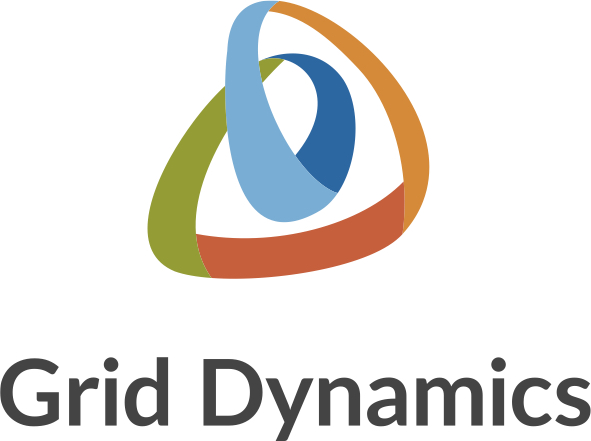
\includegraphics[scale=0.3]{gdlogo}
	\end{gdblank}
	\begin{gdblank}
		\frametitle{Hello}
		\centering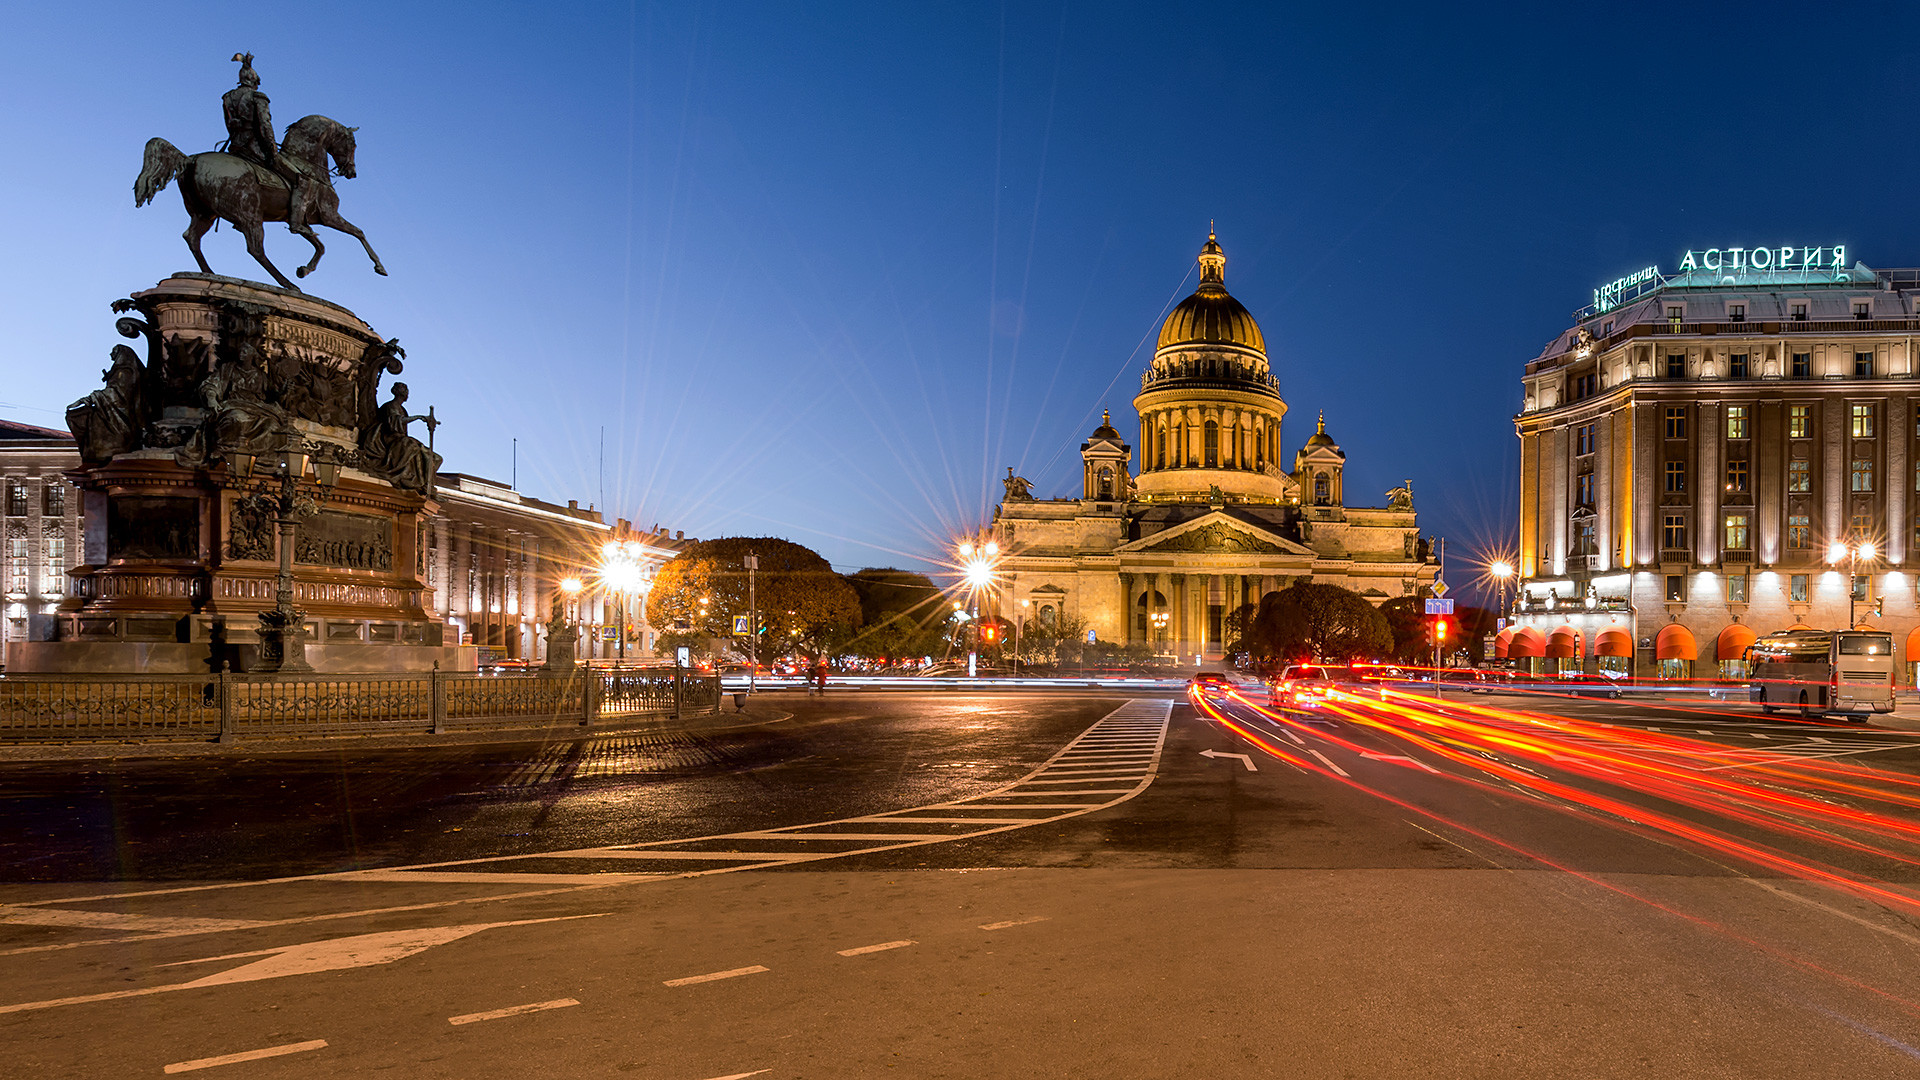
\includegraphics[scale=0.6]{spb}
		\\Saint-Petersburg
	\end{gdblank}
	\begin{gdblank}
		\frametitle{Hello}
		\centering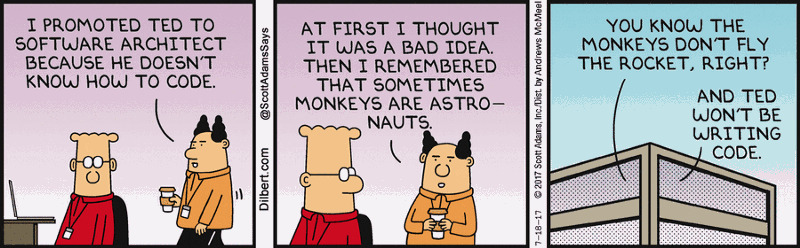
\includegraphics[scale=0.5]{arch} 
	\end{gdblank}
	\begin{gdblank}
		\frametitle{Hello}
		\centering
\includegraphics[scale=0.8]{bigdata} 
	\end{gdblank}
	\begin{gdblank}
		\frametitle{Hello}
		\begin{columns}
			\begin{column}{0.5\textwidth}
				\centering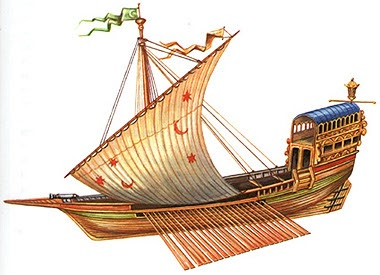
\includegraphics[scale=0.4]{galera}
			\end{column}
			\pause 
			\begin{column}{0.5\textwidth}
				\centering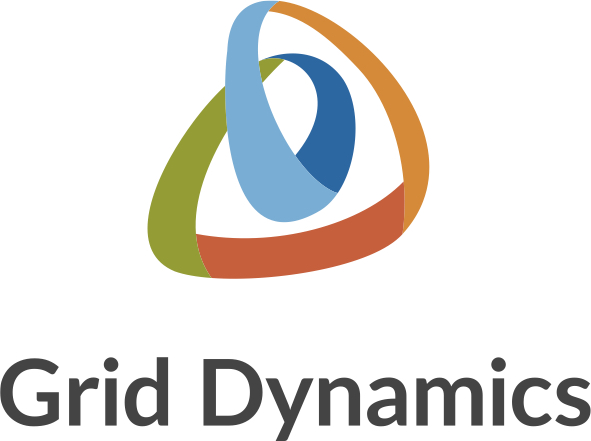
\includegraphics[scale=0.2]{gdlogo}
			\end{column}
		\end{columns}        
	\end{gdblank}
	\begin{gdblank}
		\frametitle{Time}
		\begin{columns}
			\begin{column}{0.5\textwidth}
				\centering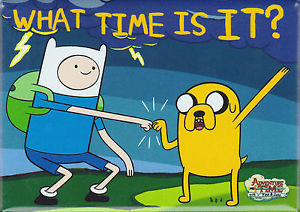
\includegraphics[scale=5]{adventuretime} 
			\end{column}
			\pause 
			\begin{column}{0.5\textwidth}
				\centering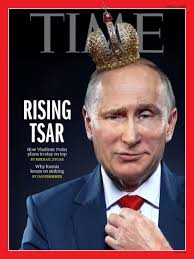
\includegraphics[scale=0.7]{timeputin} 
			\end{column}
		\end{columns}            
	\end{gdblank}
	\begin{gdblank}
		\frametitle{Time}
		\begin{columns}
			\begin{column}{0.5\textwidth}
				\centering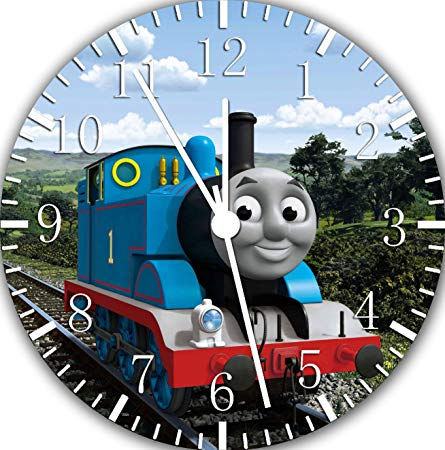
\includegraphics[scale=0.3]{thomas-train-clock} 
			\end{column}
			\pause 
			\begin{column}{0.5\textwidth}
				\centering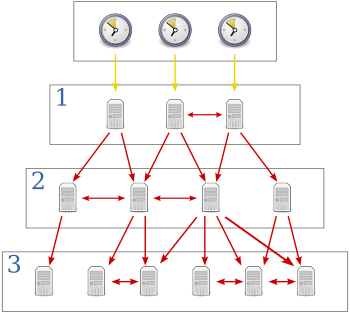
\includegraphics[scale=0.5]{strarum} 
			\end{column}
		\end{columns}            
	\end{gdblank}
	\begin{gdblankclock}
		\frametitle{Question}
		\centering\Huge What is time?           
	\end{gdblankclock} 
	\begin{gdblank}
		\frametitle{Time is ...}
		\begin{columns}
			\begin{column}{0.5\textwidth}
				\centering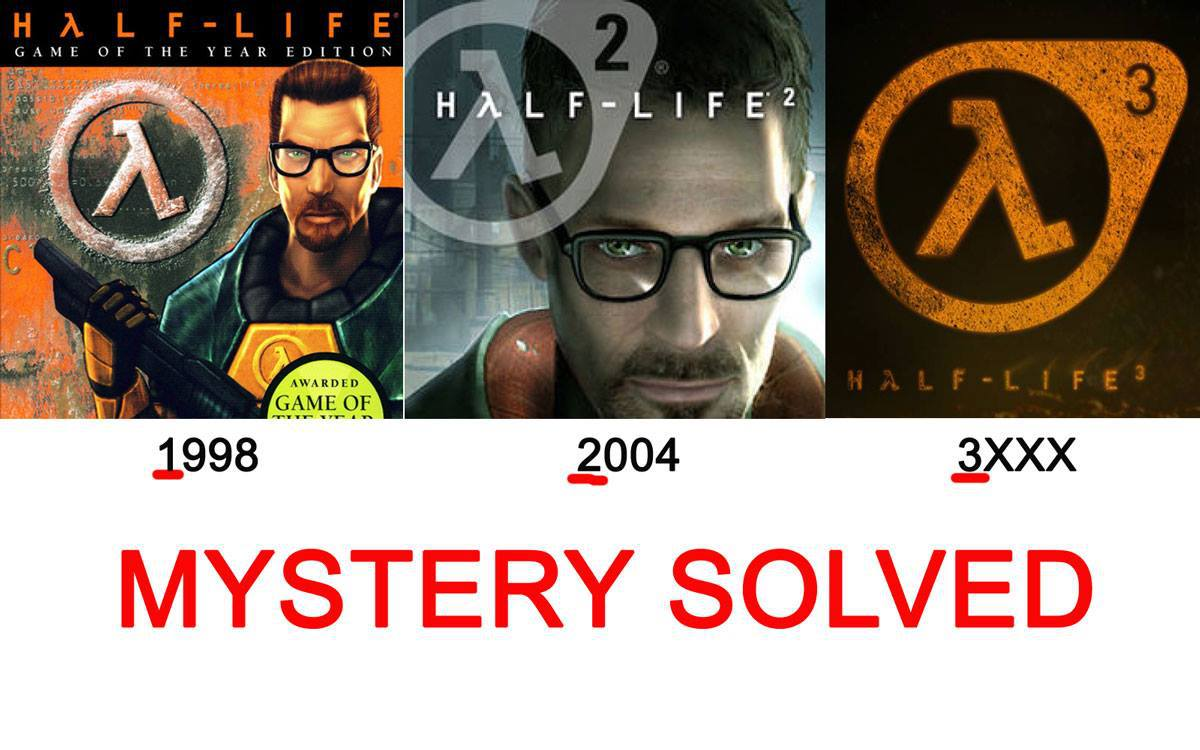
\includegraphics[scale=0.16]{halflife} 
				\\Way of arrange the order of events 
			\end{column}
			\pause 
			\begin{column}{0.5\textwidth}
				\centering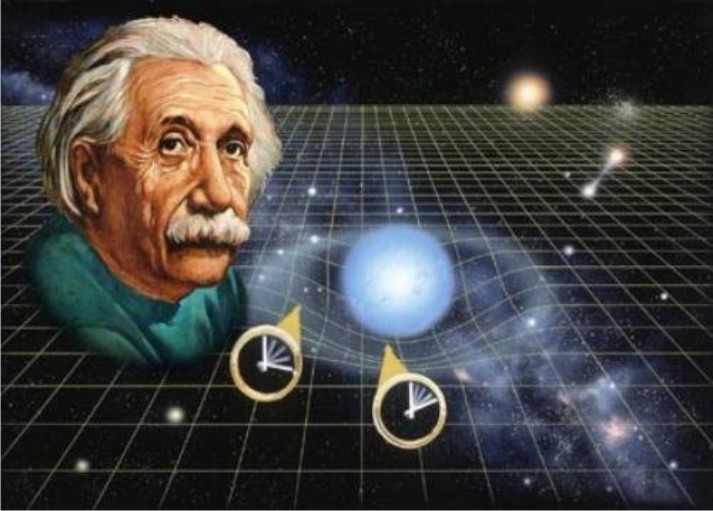
\includegraphics[scale=0.35]{einsteinspacetime} 
				\\Another dimension
			\end{column}
		\end{columns} 
	\end{gdblank} 
	\begin{gdblank}
		\frametitle{Definition of time}
		\LARGE Compact and robust definition of time has proved to be remarkably tricky and elusive.
		\large
		\vskip1cm
		\begin{itemize}
			\item What clocks measure (attr. to physicists Albert Einstein, Donald Ivey, and others)
			      \pause
			\item What prevents everything from happening at once (physicist John Wheeler and others)
			\item A linear continuum of instants (philosopher Adolf Grünbaum)
		\end{itemize}
	\end{gdblank}
	\begin{gdblank}
		\frametitle{Religion}
		\begin{columns}
			\begin{column}{0.5\textwidth}
				\centering
\includegraphics[scale=0.5]{zurvanizm} 
			\end{column}
			\begin{column}{0.5\textwidth}
				\begin{block}{Wikipedia}
					In Zurvanism, Zurvan was perceived as the god of infinite time and space and was aka ("one", "alone").
				\end{block} 
			\end{column}
		\end{columns}     
	\end{gdblank}
	\begin{gdblank}
		\frametitle{Time is ...}
		\LARGE\centering Time is something we deal with every day, and something that everyone thinks they 
		\bf understand
	\end{gdblank} 
	\begin{gdblank}
		\frametitle{Game Time}
		\Huge\centering Let's play a game
	\end{gdblank} 
	\begin{gdblank}
		\frametitle{Round 1}    
		\begin{columns}
			\begin{column}{0.70\textwidth}
				\LARGE There are always 24 hours in a day 
				\pause     
			\end{column}
			\begin{column}{0.3\textwidth}
				\large\centering Daylight saving time 
				\vskip0.5cm
				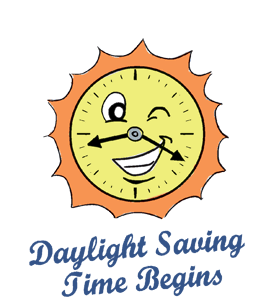
\includegraphics[scale=0.5]{daylightsaving}
			\end{column}
		\end{columns}
	\end{gdblank} 
	\begin{gdblank}
		\frametitle{Round 2}    
		\begin{columns}
			\begin{column}{0.70\textwidth}
				\LARGE A month always ends in the same year it started
				\pause     
			\end{column}
			\begin{column}{0.3\textwidth}
				\large\centering 
				\begin{itemize}
					\item Fiscal year/calendar
					\item Chinese Year
				\end{itemize}
				\vskip0.5cm
				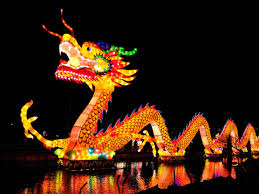
\includegraphics[scale=0.5]{china}
			\end{column}
		\end{columns}
	\end{gdblank} 
	\begin{gdblank}
		\frametitle{Round 3}    
		\begin{columns}
			\begin{column}{0.70\textwidth}
				\LARGE Months have either 28, 29, 30 or 31 days
				\pause     
			\end{column}
			\begin{column}{0.3\textwidth}
				\large\centering  September 1752 had 19 days in British Empire
				\vskip0.5cm
				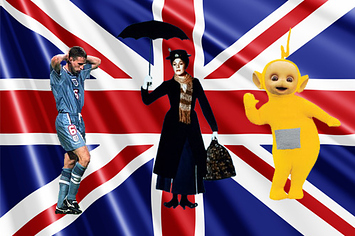
\includegraphics[scale=0.35]{british}
			\end{column}
		\end{columns}
	\end{gdblank} 
	\begin{gdblank}
		\frametitle{Everyone do it wrong!?}
		\pause
		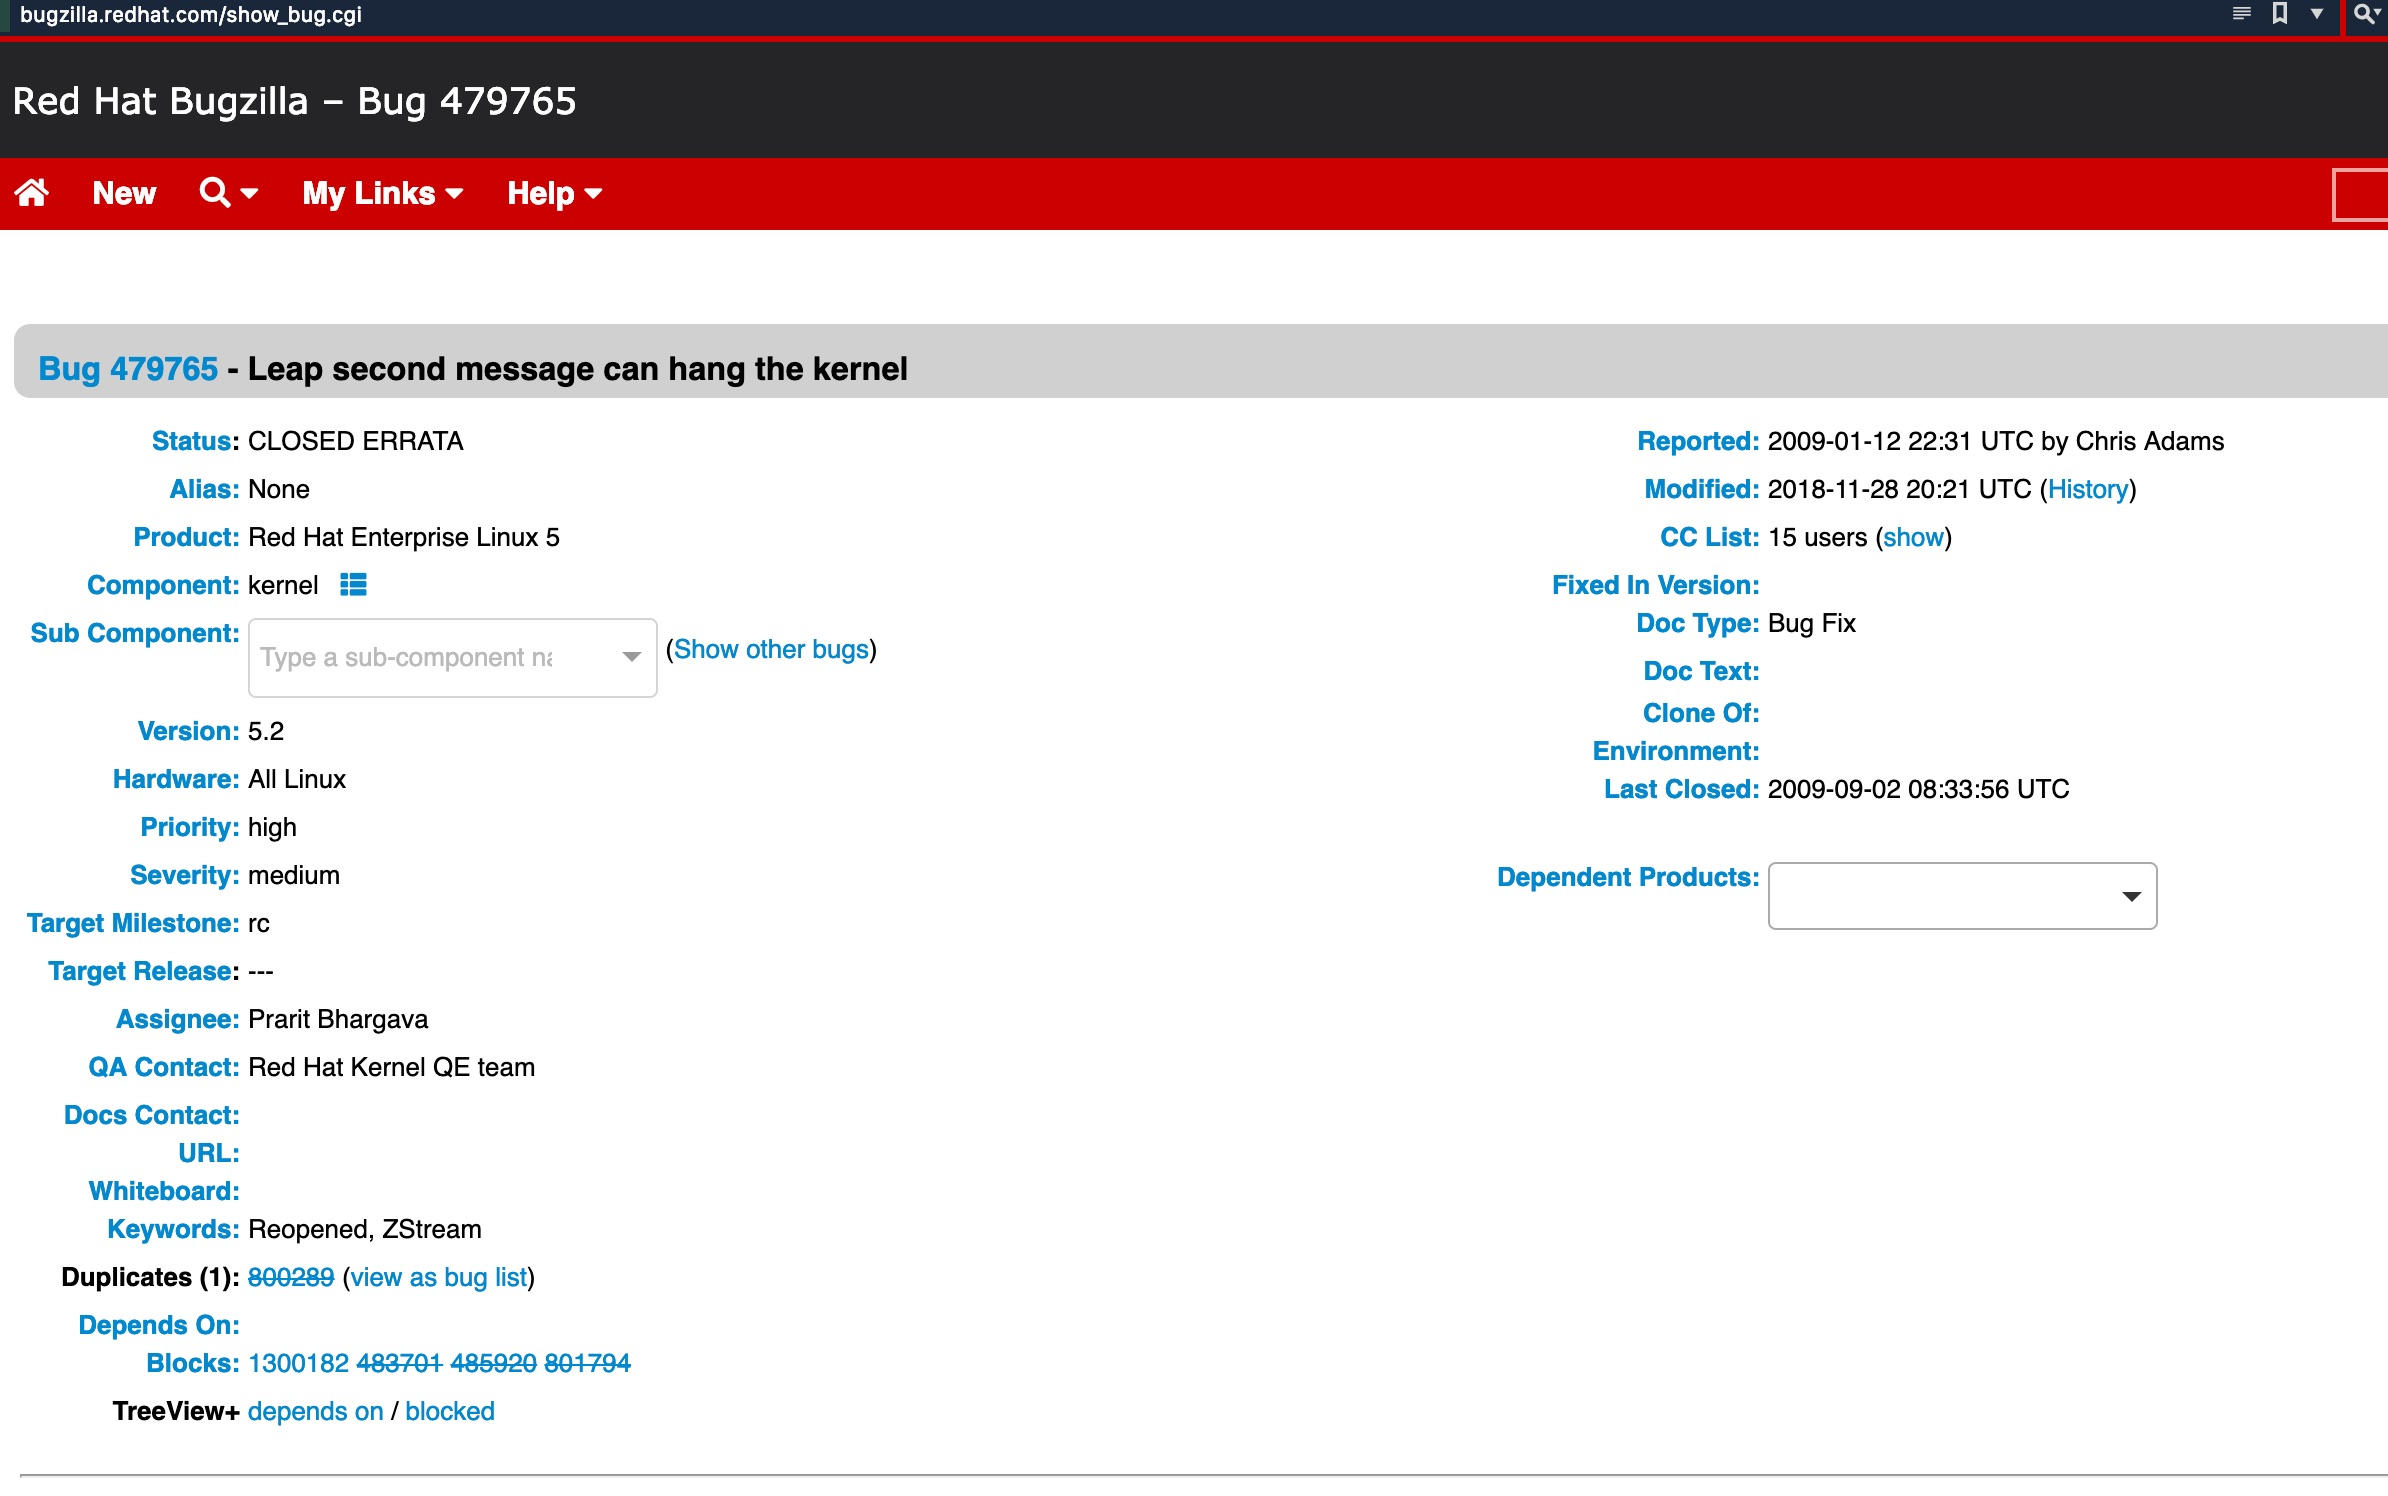
\includegraphics[width=\textwidth]{kernel-time-bug}
	\end{gdblank}   
	\begin{gdblank}
		\frametitle{Everyone do it wrong!?}
		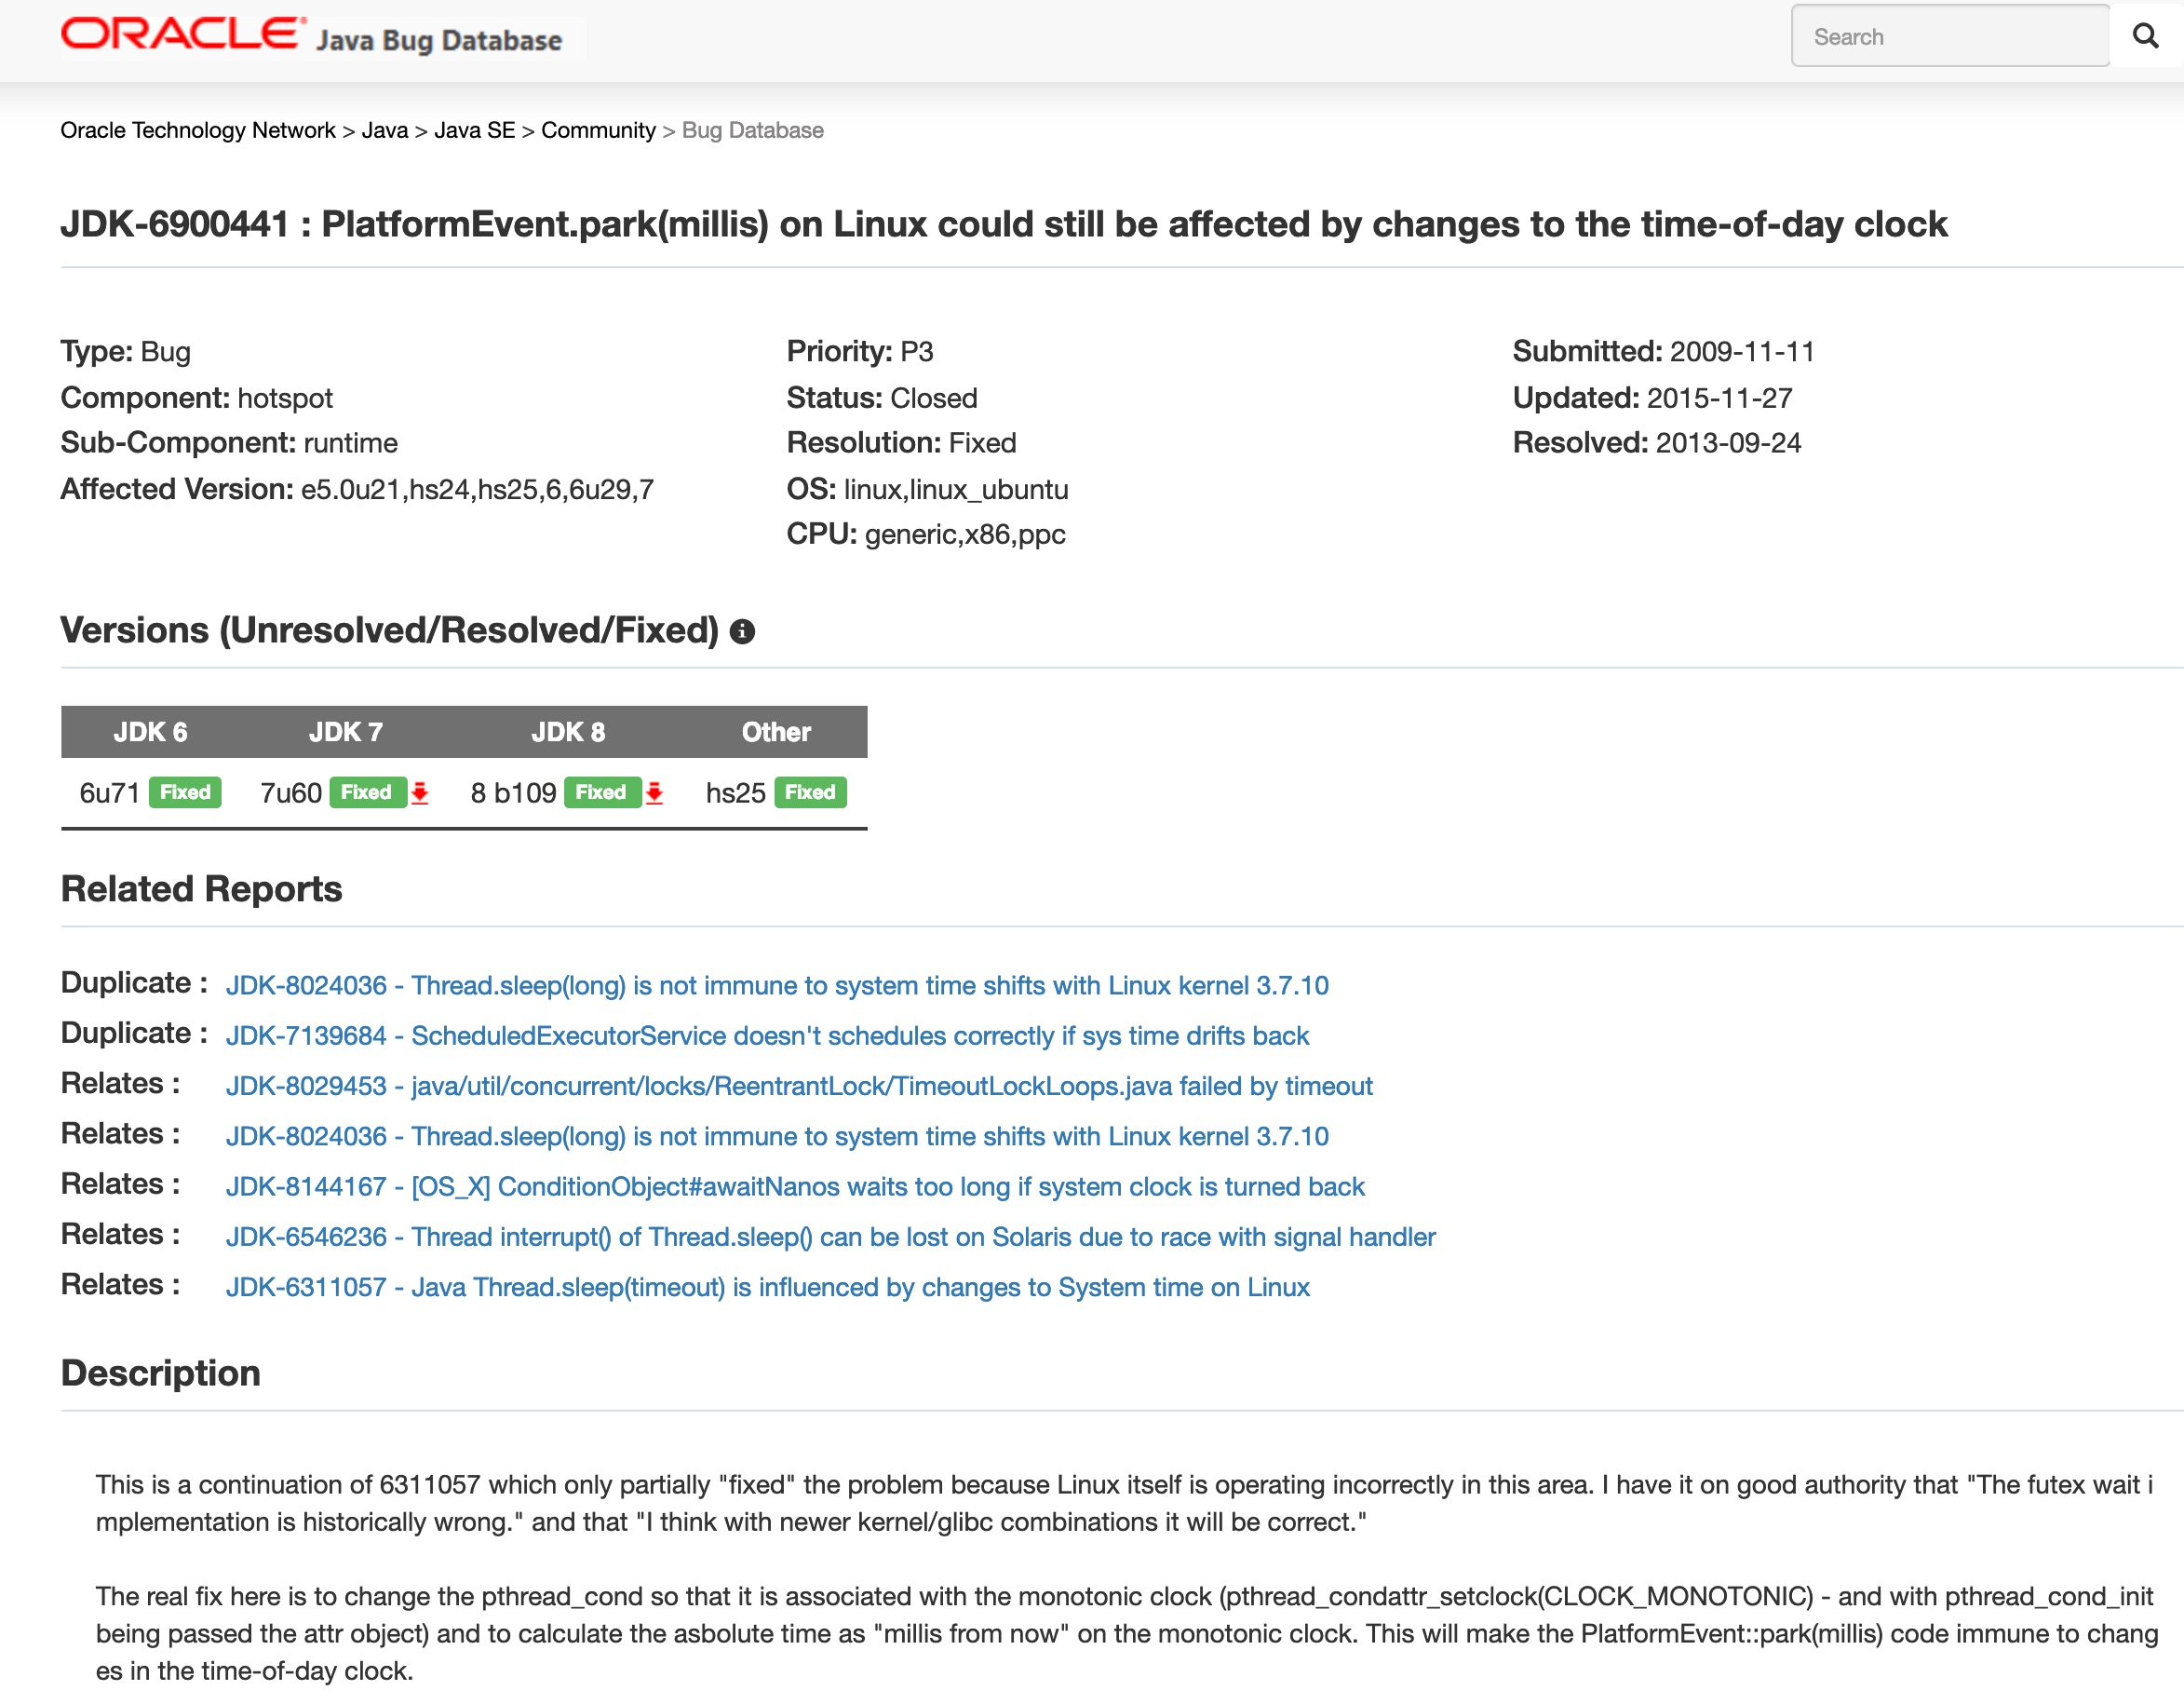
\includegraphics[width=\textwidth]{jvm-time-bug}
	\end{gdblank}
	\begin{gdblank}
		\frametitle{Distributed environment}
		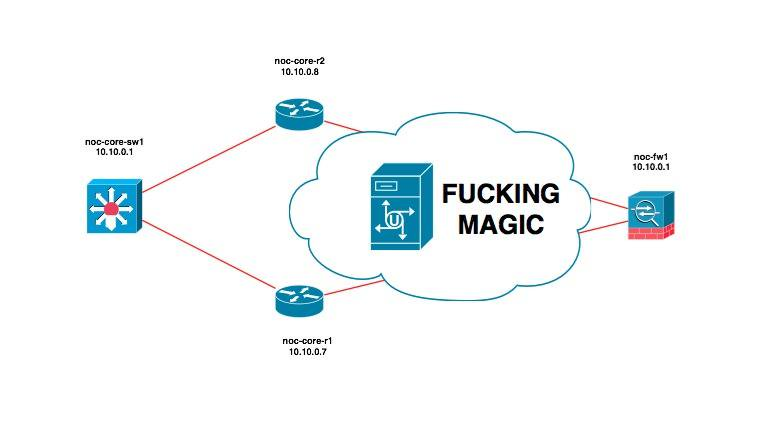
\includegraphics[width=\textwidth]{network}
	\end{gdblank}   
	
	\begin{gdblank}
		\frametitle{}
		\begin{columns}
			\begin{column}{0.5\textwidth}
			\end{column}
			\pause
			\begin{column}{0.5\textwidth}
			\end{column}
		\end{columns} 
	\end{gdblank} 
\end{document}
% There is no one simple definition of time. Time is something we deal with every day, and something that everyone thinks they understand.
% What is the time?
% Time is a way to order a set of events? % Half life 3
% Einstein Space-Time
% We don't know exactly what the time is
% That's why religions as Zurvanizm apear
% But we take this as ordered
% Okey Falsehoods programmers believe about time
% There are always 24 hours in a day.
% Years have 365 days.
% Ok, that’s not true. But at least the time zone in which a program has to run will never change.
% The system clock will always be set to a time that is not wildly different from the correct local time.
% Time has no beginning and no end. Wiki The Year 2038 problem relates to representing time in many digital systems as the number of seconds passed since 1 January 1970 and storing it as a signed 32-bit binary integer.
% Time stamps will always have the same level of precision.
% A timestamp represents the time that an event actually occurred.
% Minute could be longer than an hour 
% The same month has the same number of days in it everywhere!
% Unix time is the number of seconds since Jan 1st 1970.
% You can wait for the clock to reach exactly HH:MM:SS by sampling once a second.
% The software will never run on a space ship that is orbiting a black hole.
% September 1752 had 19 days in British Empire
% doesn't a month always end in the same year it started? 

% Even JVM and Linux are bad
% Move to distributed system. What is simultanious
% Time-Space relativity
% Cake is lie
% Ok, what we have
% Physical Clocks
% With the timer we can define: simultaneous: all actions that happen between clock ticks before: an operation that happens in a previous clock tick after: an operation that happens in a subsequent clock tick
% Multiple systems - clock skew. On any two given computers, the drift rate will likely differ.
% To solve this problem, clock synchronization algorithms are necessary.
% Clocks sync overview
% Negative time correction?
% It is not important that all processes agree on what the actual time is, but that they agree on the order in which events occur.
% Lampard Clocks - The important contribution of Lamport is that in a distributed system, clocks need not be synchronized absolutely.
% Lampard Happens Before - Defines a relationship called “happens-before”. a -> b is read as “a happens before b” 
% That's how mafia works
% Vector Clocks
% We can use this capability to build a truly distributed dataflow graph with dependencies without having a centralized coordinating process.
% Cassandra


% http://books.cs.luc.edu/distributedsystems/clocks.html#time-and-computation
% https://bugs.java.com/bugdatabase/view_bug.do?bug_id=6900441
% https://bbossola.wordpress.com/2013/09/04/jvm-issue-concurrency-is-affected-by-changing-the-date-of-the-system/
% http://yourcalendricalfallacyis.com/
% https://news.ycombinator.com/item?id=4128208
% https://infiniteundo.com/post/25326999628/falsehoods-programmers-believe-about-time#_=_
